\documentclass[12pt,letterpaper]{article}
\usepackage[utf8]{inputenc}
\usepackage[spanish]{babel}
\usepackage{graphicx}
\usepackage[left=2cm,right=2cm,top=2cm,bottom=2cm]{geometry}
\usepackage{graphicx} % figuras
% \usepackage{subfigure} % subfiguras
\usepackage{float} % para usar [H]
\usepackage{amsmath}
\usepackage{minted}
%\usepackage{txfonts}
\usepackage{stackrel} 
\usepackage{multirow}
\usepackage{enumerate} % enumerados
\renewcommand{\labelitemi}{$-$}
\renewcommand{\labelitemii}{$\cdot$}
% \author{}
% \title{Caratula}
\begin{document}

% Fancy Header and Footer
% \usepackage{fancyhdr}
% \pagestyle{fancy}
% \cfoot{}
% \rfoot{\thepage}
%

% \usepackage[hidelinks]{hyperref} % CREA HYPERVINCULOS EN INDICE

% \author{}
\title{Caratula}

\begin{titlepage}
\begin{center}
\large{UNIVERSIDAD PRIVADA DE TACNA}\\
\vspace*{-0.025in}
\begin{figure}[htb]
\begin{center}

\includegraphics[width=8cm]{./images/logo}
\end{center}
\end{figure}
\vspace*{0.15in}
INGENIERIA DE SISTEMAS  \\

\vspace*{0.5in}
\begin{large}
TITULO:\\
\end{large}

\vspace*{0.1in}
\begin{Large}
\textbf{INFORME DE LABORATORIO N 06} \\
\end{Large}

\vspace*{0.3in}
\begin{Large}
\textbf{CURSO:} \\
\end{Large}

\vspace*{0.1in}
\begin{large}
BASE DE DATOS II\\
\end{large}

\vspace*{0.3in}
\begin{Large}
\textbf{DOCENTE(ING):} \\
\end{Large}

\vspace*{0.1in}
\begin{large}
 Patrick Cuadros Quiroga\\
\end{large}

\vspace*{0.2in}
\vspace*{0.1in}
\begin{large}
Integrantes: \\
\begin{flushleft}
Moreno Mulluni Luis Angel		\hfill	(2017057864) \\
Layme Valeriano Diego 		\hfill	(2017057865) \\
Mamani Calisaya Yonathan 	           	\hfill	(2017057863) \\
\end{flushleft}
\end{large}
\end{center}

\end{titlepage}


\tableofcontents % INDICE
\thispagestyle{empty} % INDICE SIN NUMERO
\newpage
\setcounter{page}{1} % REINICIAR CONTADOR DE PAGINAS DESPUES DEL INDICE DE CUESTIONARIO

\section{Pregunta 01 – ¿Qué sucede al ejecutar los siguientes comandos?} 

\begin{enumerate}
\item  STARTUP OPEN\\
Inicia la instancia, monte y abra la base de datos. Esto se puede hacer en modo no restringido, permitiendo el acceso a todos los usuarios, o en modo restringido, permitiendo el acceso solo para administradores de bases de datos.
\item  STARTUP MOUNT\\
Inicia la instancia y monte la base de datos, pero déjela cerrada. Este estado permite ciertas actividades de DBA, pero no permite el acceso general a la base de datos.
\item  STARTUP NOMOUNT\\
Inicia la instancia sin montar una base de datos. Esto no permite el acceso a la base de datos y, por lo general, se haría solo para la creación de la base de datos o la recreación de archivos de control.
\item  STARTUP FORCE\\
Obliga a la instancia a iniciarse después de un problema de inicio o apagado.
\item  STARTUP RESTRICT\\
Puede iniciar una instancia y, opcionalmente, montar y abrir una base de datos, en modo restringido, de modo que la instancia solo esté disponible para el personal administrativo (no para usuarios de bases de datos generales).
\item  STARTUP RECOVER\\
Inicie la instancia y haga que la recuperación completa de los medios comience de inmediato.
\item  SHUTDOWN NORMAL\\
Para cerrar una base de datos en situaciones normales, use el comando shutdown con la cláusula normal
\item  SHUTDOWN TRANSACTIONAL\\
Cuando desee realizar un cierre planificado de una instancia mientras permite que las transacciones activas se completen primero, use el comando shutdown con la cláusula transaccional.
\item  SHUTDOWN ABORT\\
Cuando deba cerrar una base de datos abortando transacciones y conexiones de usuario, ejecute el comando shutdown con la cláusula de cancelación
\item  SHUTDOWN INMEDIATE\\
Para cerrar una base de datos inmediatamente, use el comando shutdown con la cláusula inmediata.
\end{enumerate}
\section{Pregunta 02 – En el script lab\_02\_01.sql, se establecen privilegios de sistema, enliste los privilegios de sistema (DDL) utilizados y describa cada uno de ellos. } 


\begin{enumerate}
\item GRANT CREATE ANY CLUSTER TO "DBA1";
\\ Permite crear clusteres
\item GRANT CREATE ANY CONTEXT TO "DBA1";
\\  permite crear contextos
\item GRANT CREATE ANY DIMENSION TO "DBA1";
\\  permite  crear dimensiones
\item GRANT CREATE ANY DIRECTORY TO "DBA1";
\\  permite crear directorios
\item GRANT CREATE ANY EVALUATION CONTEXT TO "DBA1" WITH ADMIN OPTION;
\\  permite evaluar contextos
\item GRANT CREATE ANY INDEX TO "DBA1";
\\  permite crear indices
\item GRANT CREATE ANY INDEXTYPE TO "DBA1";
\\  permite crear todos los tipos de indices
\item GRANT CREATE ANY JOB TO "DBA1";
\\  permite crear jobs
\item GRANT CREATE ANY LIBRARY TO "DBA1";
\\  permite crear librerias a nivel de esquema general
\item GRANT CREATE ANY MATERIALIZED VIEW TO "DBA1";
\\  permite vistas materializadas a nivel de esquema general
\item GRANT CREATE ANY OPERATOR TO "DBA1";
\\  permite crear operaciones a nivel de esquema general
\item GRANT CREATE ANY OUTLINE TO "DBA1";
\\  permite crear outlines a nivel de esquema general
\item GRANT CREATE ANY PROCEDURE TO "DBA1";
\\  permite crear procedimientos a nivel de esquema general
\item GRANT CREATE ANY RULE TO "DBA1" WITH ADMIN OPTION;
\\  permite crear reglas a nivel de esquema general
\item GRANT CREATE ANY RULE SET TO "DBA1" WITH ADMIN OPTION;
\\  permite modificar reglas a nivel de esquema general
\item GRANT CREATE ANY SEQUENCE TO "DBA1";
\\  permite crear secuencias a nivel de esquema general
\item GRANT CREATE ANY SQL PROFILE TO "DBA1";
\\  permite crear perfiles sql a nivel de esquema general
\item GRANT CREATE ANY SYNONYM TO "DBA1"; 
\\ permite crear sinonimos para tablas , vistas , secuencia , profecimiento , function almacenada , paquete , vista materializada ,  objeto de esquema y tipo definido  por el usuario a nivel de esquema general
\item GRANT CREATE ANY TABLE TO "DBA1";
\\  permite crear tablas a nivel de esquema general
\item GRANT CREATE ANY TRIGGER TO "DBA1";
\\  permite crear triggers a nivel de esquema general
\item GRANT CREATE ANY TYPE TO "DBA1";
\\  permite crear types a nivel de esquema general
\item GRANT CREATE ANY VIEW TO "DBA1";
\\  permite crear vistas a nivel de esquema general
\item GRANT CREATE CLUSTER TO "DBA1";
\\  permite crear cluster a nivel de su propio esquema
\item GRANT CREATE DATABASE LINK TO "DBA1";
\\  permite crear database link a nivel de su propio esquema
\item GRANT CREATE DIMENSION TO "DBA1";
\\  permite crear dimensiones a nivel de su propio esquema
\item GRANT CREATE EVALUATION CONTEXT TO "DBA1" WITH ADMIN OPTION;
\\ permite crear un contexto de evaluacion como si fuera usuario de nivel administrador
\item GRANT CREATE EXTERNAL JOB TO "DBA1";
\\ permite crear un JOB externo
\item GRANT CREATE INDEXTYPE TO "DBA1";
\\ permite crear diferentes tipos de indices
\item GRANT CREATE JOB TO "DBA1";
\\ permite crear JOB 
\item GRANT CREATE LIBRARY TO "DBA1";
\\ permite crear librerias
\item GRANT CREATE MATERIALIZED VIEW TO "DBA1";
\\permite crear vistas MATERIALED 
\item GRANT CREATE OPERATOR TO "DBA1";
\\ permite crear operadores
\item GRANT CREATE PROCEDURE TO "DBA1";
\\permite crear procedimientos almacenados
\item GRANT CREATE PROFILE TO "DBA1";
\\permite crear perfiles
\item GRANT CREATE PUBLIC DATABASE LINK TO "DBA1";
\\permite crear crear enlaces publicos a objetos de la base de datos
\item GRANT CREATE PUBLIC SYNONYM TO "DBA1";
\\permite crear sinonimos publicos a las tablas
\item GRANT CREATE ROLE TO "DBA1";
\\permite crear roles
\item GRANT CREATE ROLLBACK SEGMENT TO "DBA1";
\\permite crear segmentos de rollback
\item GRANT CREATE RULE TO "DBA1" WITH ADMIN OPTION;
\\permite crear reglas con un nivel de administrador
\item GRANT CREATE RULE SET TO "DBA1" WITH ADMIN OPTION;
\\permite crear conjunto de reglas con un nivel de administrador
\item GRANT CREATE SEQUENCE TO "DBA1";
\\permite crear secuencias
\item GRANT CREATE SESSION TO "DBA1";
\\permite crear sesiones
\item GRANT CREATE SYNONYM TO "DBA1";
\\permite crear sinonimos
\item GRANT CREATE TABLE TO "DBA1";
\\permite crear tablas
\item GRANT CREATE TABLESPACE TO "DBA1";
\\permite crear tablas de espacio
\item GRANT CREATE TRIGGER TO "DBA1";
\\permite crear TRIGGER
\item GRANT CREATE TYPE TO "DBA1";
\\permite crear TYPE
\item GRANT CREATE USER TO "DBA1";
\\permite crear usuarios
\item GRANT CREATE VIEW TO "DBA1";
\\permite crear vistas
\item GRANT ALTER ANY CLUSTER TO "DBA1";
\\permite modificar cualquier cluster
\item GRANT ALTER ANY DIMENSION TO "DBA1";
\\permite modificar cualquier dimension
\item GRANT ALTER ANY EVALUATION CONTEXT TO "DBA1" WITH ADMIN OPTION;
\\permite modificar cualquier contexto de evaluacion con un nivel administrador
\item GRANT ALTER ANY INDEX TO "DBA1";
\\permite modificar cualquier indice
\item GRANT ALTER ANY INDEXTYPE TO "DBA1";
\\permite modificar cualquier tipo de indice
\item GRANT ALTER ANY LIBRARY TO "DBA1";
\\permite modificar cualquier libreria
\item GRANT ALTER ANY MATERIALIZED VIEW TO "DBA1";
\\permite modificar vistas MATERIALIZED
\item GRANT ALTER ANY OUTLINE TO "DBA1";
\\permite modificar cualquier OUTLINE
\item GRANT ALTER ANY PROCEDURE TO "DBA1";
\\permite modificar cualquier procedimiento almacenado
\item GRANT ALTER ANY ROLE TO "DBA1";
\\permite modificar cualquier rol
\item GRANT ALTER ANY RULE TO "DBA1" WITH ADMIN OPTION;
\\permite modificar cualquier regla con un nivel de administrador
\item GRANT ALTER ANY RULE SET TO "DBA1" WITH ADMIN OPTION;
\\permite modificar cualquier conjunto de reglas
\item GRANT ALTER ANY SEQUENCE TO "DBA1";
\\permite modificar cualquier secuencia
\item GRANT ALTER ANY SQL PROFILE TO "DBA1";
\\permite modificar cualquier perfil sql
\item GRANT ALTER ANY TABLE TO "DBA1";
\\permite modificar cualquier tabla
\item GRANT ALTER ANY TRIGGER TO "DBA1";
\\permite modificar cualquier TRIGGER
\item GRANT ALTER ANY TYPE TO "DBA1";
\\permite modificar cualquier TYPE
\item GRANT ALTER DATABASE TO "DBA1";
\\permite modificar la base de datos
\item GRANT ALTER PROFILE TO "DBA1";
\\permite modificar  perfiles
\item GRANT ALTER RESOURCE COST TO "DBA1";
\\permite modificar recurso de formula de costo
\item GRANT ALTER ROLLBACK SEGMENT TO "DBA1";
\\permite modificar segmento de rollback
\item GRANT ALTER SESSION TO "DBA1";
\\permite modificar sesiones
\item GRANT ALTER SYSTEM TO "DBA1";
\\permite modificar a SYSTEM
\item GRANT ALTER TABLESPACE TO "DBA1";
\\permite modificar una tabla de espacio
\item GRANT ALTER USER TO "DBA1";
\\permite modificar usuarios
\item GRANT DROP ANY CLUSTER TO "DBA1";
\\permite eliminar cualquier cluster
\item GRANT DROP ANY CONTEXT TO "DBA1";
\\permite eliminar cualquier contexto
\item GRANT DROP ANY DIMENSION TO "DBA1";
\\permite eliminar cualquier dimension
\item GRANT DROP ANY DIRECTORY TO "DBA1";
\\permite eliminar cualquier directorio
\item GRANT DROP ANY EVALUATION CONTEXT TO "DBA1" WITH ADMIN OPTION;
\\permite eliminar cualquier contexto de evaluacion con un nivel de administrador
\item GRANT DROP ANY INDEX TO "DBA1";
\\permite eliminar cualquier indice
\item GRANT DROP ANY INDEXTYPE TO "DBA1";
\\permite eliminar cualquier tipo de indice
\item GRANT DROP ANY LIBRARY TO "DBA1";
\\permite eliminar cualquier libreria
\item GRANT DROP ANY MATERIALIZED VIEW TO "DBA1";
\\permite eliminar cualquier vista MATERIALIZED
\item GRANT DROP ANY OPERATOR TO "DBA1";
\\permite eliminar cualquier operador
\item GRANT DROP ANY OUTLINE TO "DBA1";
\\permite eliminar cualquier OUTLINE
\item GRANT DROP ANY PROCEDURE TO "DBA1";
\\permite eliminar cualquier procedimiento almacenado
\item GRANT DROP ANY ROLE TO "DBA1";
\\permite eliminar cualquier rol
\item GRANT DROP ANY RULE TO "DBA1" WITH ADMIN OPTION;
\\permite eliminar cualquier regla con un nivel de administrador
\item GRANT DROP ANY RULE SET TO "DBA1" WITH ADMIN OPTION;
\\permite eliminar cualquier conjunto de reglas con un nivel de administrador
\item GRANT DROP ANY SEQUENCE TO "DBA1";
\\permite eliminar cualquier secuencia
\item GRANT DROP ANY SQL PROFILE TO "DBA1";
\\permite eliminar cualquier perfil sql
\item GRANT DROP ANY SYNONYM TO "DBA1";
\\permite eliminar cualquier sinonimo de tabla
\item GRANT DROP ANY TABLE TO "DBA1";
\\permite eliminar cualquier tabla
\item GRANT DROP ANY TRIGGER TO "DBA1";
\\permite eliminar cualquier TRIGGER
\item GRANT DROP ANY TYPE TO "DBA1";
\\permite eliminar cualquier TYPE
\item GRANT DROP ANY VIEW TO "DBA1";
\\permite eliminar cualquier vista
\item GRANT DROP PROFILE TO "DBA1";
\\permite eliminar perfiles
\item GRANT DROP PUBLIC DATABASE LINK TO "DBA1";
\\permite eliminar enlaces publicos de bases de datos
\item GRANT DROP PUBLIC SYNONYM TO "DBA1";
\\permite eliminar sinonimos publicos
\item GRANT DROP ROLLBACK SEGMENT TO "DBA1";
\\permite eliminar segmentos de rollback
\item GRANT DROP TABLESPACE TO "DBA1";
\\permite eliminar tablas de espacio
\item GRANT DROP USER TO "DBA1";
\\permite eliminar usuarios
\end{enumerate}
\section{Pregunta 03 – Enliste y describa los tipos de TableSpace que existen en Oracle}
Ejecutamos el siguiente comando
\begin{minted}{sql}
    SELECT TABLESPACE_NAME ,CONTENTS FROM DBA_TABLESPACES
\end{minted}

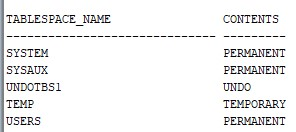
\includegraphics[width=8cm]{./images/tablespace}


\begin{enumerate}
    \item Permanente (PERMANENT) \\
Utiliza espacios de tabla permanentes para almacenar sus datos de usuario y aplicación. La base de datos Oracle utiliza espacios de tabla permanentes para almacenar datos permanentes, como los datos del sistema. A cada usuario se le asigna un espacio de tabla permanente predeterminado.

\item Deshacer (UNDO)\\

Una base de datos que se ejecuta en el modo de administración automática de deshacer crea y administra de forma transparente los datos de deshacer en el espacio de tablas de deshacer. La base de datos Oracle utiliza los datos de deshacer para revertir las transacciones, para proporcionar coherencia de lectura, para ayudar con la recuperación de la base de datos y para habilitar funciones como Oracle Flashback Query. Una instancia de base de datos solo puede tener un espacio de tablas de deshacer activo.

\item Temporal (TEMPORARY)\\

Los espacios de tabla temporales se utilizan para almacenar datos temporales, como se crearía cuando las sentencias de SQL realicen operaciones de clasificación. Una base de datos Oracle obtiene un espacio de tabla temporal cuando se crea la base de datos. Si estuviera creando un grupo de espacio de tablas temporal, crearía otro espacio de tabla temporal.
\end{enumerate}





\end{document}